\section{Aufbau}
\label{sec:Aufbau und Justage}

Eine schematische Skizze der Apparatur ist in
Abbildung \ref{fig:aufbau} dargestellt.

Um das Sagnac-Interferometer zu justieren wurde
zunächst der Spiegel $\symup{M}_{\text{A}}$ mithilfe von M1
und M2 und dem PBSC\footnote{polarizing beam
splitter cube $\hat{=}$ Strahlteiler} so justiert,
dass der Strahl durch das mittlere Loch der
zweier Blenden läuft. Diese beiden Blenden sind
hierfür einmal hinter dem Strahlteiler und einmal
vor $\symup{M}_{\text{A}}$ positioniert.
Dabei wird der vom PBSC abgelenkte Strahl derweil
blockiert.
\\
Zur Justage des Spiegels $\symup{M}_{\text{C}}$ werden die Blenden an
die Positionen 8 und 9 versetzt und durch drehen des
Strahlteilers der Strahl durch die mittleren Löcher
der Blenden gelenkt.
Hierbei sollte der durchgehende Strahl vom PBSC
blockiert werden.
\\
Zur Justage von Spiegel $\symup{M}_{\text{B}}$ werden die Blenden an
die Positionen 5 und 6 verlegt und durch drehen der
Bodenplatte von $M_{\text{B}}$ der von $M_{\text{A}} (M_{\text{C}})$
kommende Strahl durch die mittleren Löcher gelenkt.
Dies wird für den gegenläufigen Strahl wiederholt
bis sich die beiden Strahlen in einem Punkt auf dem
PBSC treffen.
\\
Auf einem Schirm hinter dem PBSC kann nun das
Interferenzmuster betrachtet werden, nachdem ein
um $\SI{45}{\degree}$ gedrehter Polarisationsfilter
eingebaut wird.
Weist das Interferenzmuster Streifen auf, muss
nachjustiert werden bis die Streifen verschwinden.
Im Anschluss wird der Strahl so verschoben, dass er
durch das äußere Loch der Blende an Position 2
läuft. Die Strahlen sollten nun durch je eine der
beiden Glasplatten laufen, sodass sie unabhängig
voneinander manipuliert werden können.

\begin{figure}
    \centering
    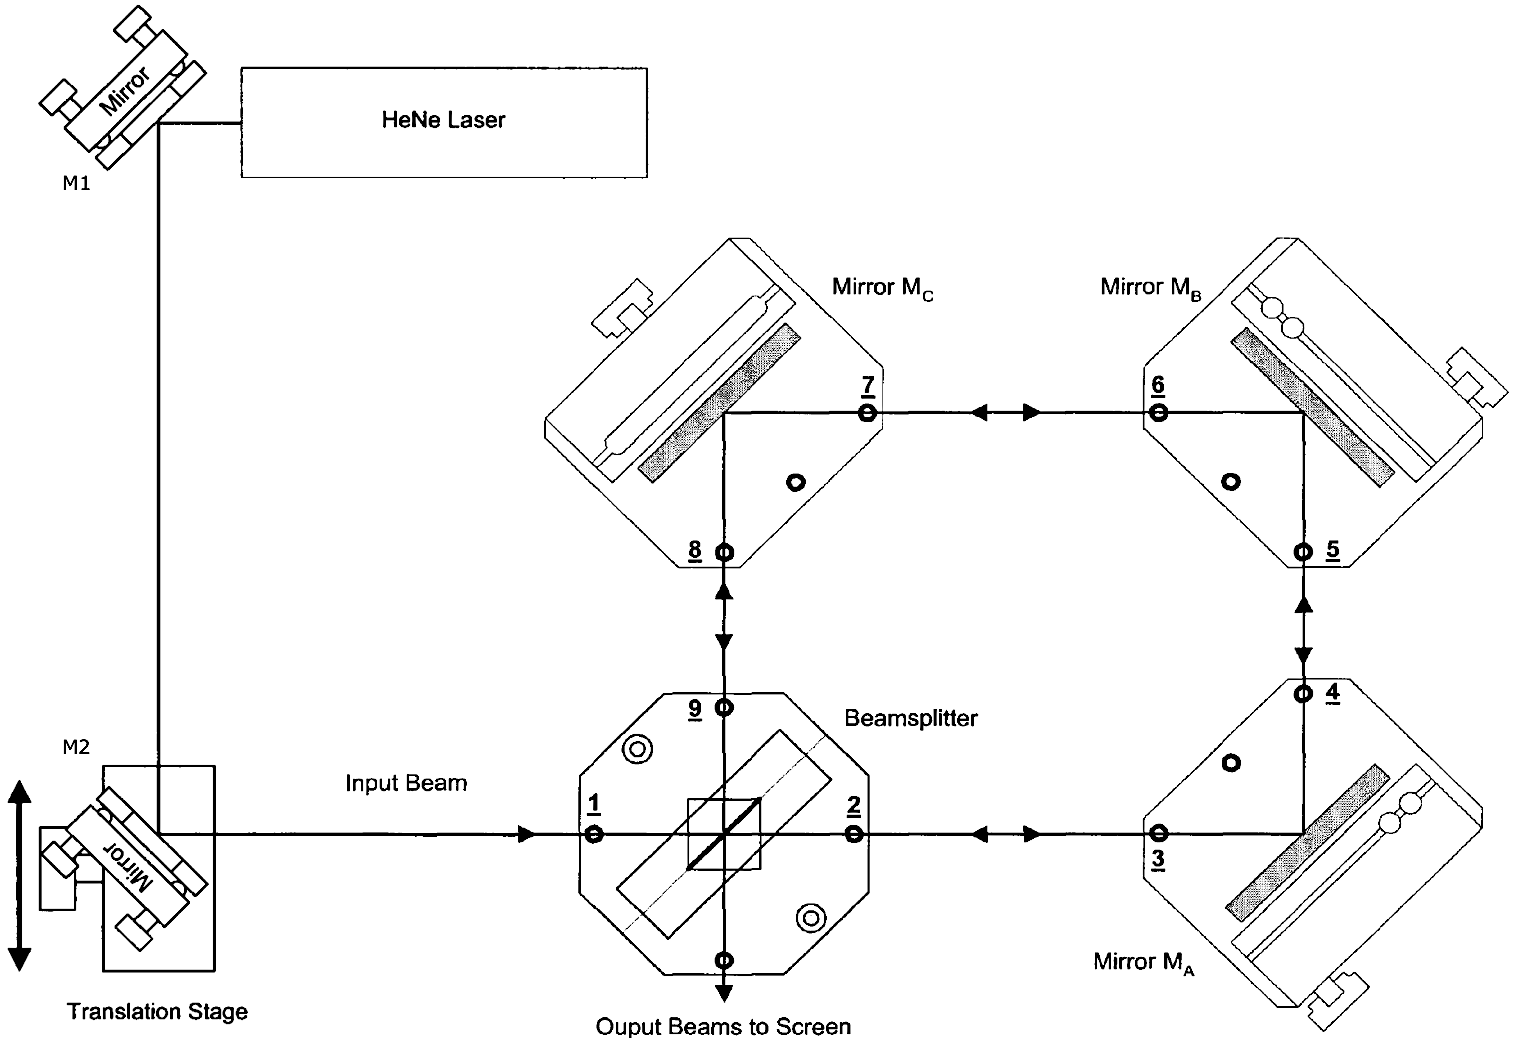
\includegraphics[width=0.9\textwidth]{pdf/aufbau.png}
    \caption{Aufbau des Sagnac-Interferometers.}
    \label{fig:aufbau}
\end{figure}

\section{Durchführung}
\label{sec:durchfuehrung}

Zunächst wird der Kontrast des Interferometes
bestimmt indem vor den PBSC ein Polarisationsfilter
gebaut wird. Es wird der Kontrast in
Abhängigkeit der Polarisationsrichtung des Strahls
bestimmt. Mithilfe des Doppelglashalters können die
Interferenzextrema bestimmt und somit der Kontrast
bestimmt werden.

Anschließend wird der Brechungsindex von Glas bei
maximalem Kontrast gemessen.
Dafür wird der gesamte Winkelbereich des
Doppelglasbehälters durchfahren und die
Interferenzmaxima bzw. -Minima in Abhängigkeit
des Drehwinkels $θ$ gezählt.

Die resultierende Phasenverschiebung $\Del{Φ}$
für kleine Drehwinkel bei einem Brechungsindex $n$
ergibt sich dann gemäß Gleichung \eqref{eqn:deltheta}.

Um den Brechungsindex eines Gases zu bestimmen, wird
eine Gaszelle in einem der beiden Strahlengänge
installiert. Nach der Evakuierung der Gaszelle wird
langsam und gleichmäßig Luft eingelassen und die Anzahl der
Interferenzmaxima gezählt.
